\chapter{Theory}
\section{Machine Learning}

Historically computers had to be programmed on a specific task using domain knowledge of humans. Machine learning challenges this traditional way of programming. Rather than trough extensive domain knowledge, machine learning algorithms are used to autonomously learn from data and information. 
\\
%https://www.forbes.com/sites/bernardmarr/2016/02/19/a-short-history-of-machine-learning-every-manager-should-read/#77bf286315e7

This intention is often represented by a 'learning' \emph{input-output function}. Assume there exists function, $f$, which represents a true behaviour or correlation. The task of any machine learning algorithm is thereby to find a \emph{hypothesis function} $h$ that resembles the behaviour of f as closely as possible. Both $f$ and $h$ are function of a fixed length vector-valued input $X={x_1, x_2, ... , x_n}$ which has $n$ components. Those might be $n$ attributes of an observed object. An input $x$ is often referred to as a \emph{data point}. The components of a data point are the $x$ \emph{features} of $x$. 
The features of a data point span the \emph{feature space}. The feature space refers to the $n$-dimensional space in which the features of a data point are represented.
\\
The function $h$ can be thought of as a device that has $X$ as an input and $h(X)$ as an output. The hypothesis function, h, is selected based on a trainings set, $\Xi$, of $m$ input vector examples.
\\
There are two major settings in machine learning. 

The first setting is \emph{unsupervised learning}. In this case the trainings set of vectors $\Xi$ doesn't provide information about the value $f(X)$ . The goal of the unsupervised learning algorithms usually is to partition the training set into subset, $\Xi$ \textsubscript{1}, $\Xi$ \textsubscript{2}, ..., $\Xi$ \textsubscript{r}. An example for this unsupervised machine learning learning problem is \emph{clustering.}, which desired to find ways to find clusters in data and discovery relationships in the data.

The second is  \emph{supervised learning} in which the values of $f$ for the samples in the training set $\Xi$ are known. This values of $f$ corresponding to a sample  The assumption is that a hypothesis $h$ is a good guess for $f$ when $h(X)$ agrees with the values of $f$ for the same samples.
In supervised machine learning two main areas are distinguished, \emph{Regression} and \emph{Classification}. In Regression the hypothesis $h$ has a continuous output. Regression could for instance be used to approximate a function for a stock price and predict a future stock price as a numerical value on a continuous range of possible prices.
Classification has a categorical output. Classification could be used to classify emails to either 

An example of a supervised learning problem is classification, which will be discussed in the later in this chapter in more detail.

%http://ai.stanford.edu/people/nilsson/MLBOOK.pdf 5/6/..




Data point
feature
feature space
dimensions
feature vector

\section{Classification}


classification, inpu, representation, hypotesis, generalization:
% http://cs.du.edu/~mitchell/mario_books/Introduction_to_Machine_Learning_-_2e_-_Ethem_Alpaydin.pdf 21

classification application in pattern recognition 
% http://cs.du.edu/~mitchell/mario_books/Introduction_to_Machine_Learning_-_2e_-_Ethem_Alpaydin.pdf 6

\section{Evaluation of Classifiers}
\begin{itemize}
\item{f-score}
fscore , precision, recall
% http://delivery.acm.org/10.1145/320000/312647/p42-yang.pdf?ip=134.155.178.109&id=312647&acc=ACTIVE%20SERVICE&key=2BA2C432AB83DA15%2E33B98ACB330D6FA0%2E4D4702B0C3E38B35%2E4D4702B0C3E38B35&CFID=976370719&CFTOKEN=43508633&__acm__=1503605339_b0f297be35db501d0410685c60e0b4b6
(2 oben rechts)
\item{Cross validation}
% https://wiki.eecs.yorku.ca/course_archive/2014-15/F/4412/_media/ensemble_data_mining.pdf 26 (44)

especially k-fold validation: 
is non exhaustive

% http://ai.stanford.edu/people/nilsson/MLBOOK.pdf  82

\end{itemize}
\section{Algorithms}
\begin{itemize}
\item{hyper-parameters}
% http://jmlr.csail.mit.edu/papers/volume13/bergstra12a/bergstra12a.pdf 2
\end{itemize}
\subsection{Linear support vector classifier}
In this chapter the support vector classifier will be introduced. The method was developed in the 1990’s and is often used as one of the best performing 'out of the box' classifiers. The support vector classifier is a extension of a maximal margin classifier. First  the concept of classification using a hyperplane and with a maximal margin classifier will be explained. Then the extension to a support vector classifier will be shown.

\subsubsection{Hyperplane classification}
The goal of the maximal margin classifier is to classify data by finding a hyperplane that optimally separates two classes in a dataset. 
\\
A hyperplane is a flat affine subspace of dimension $p-1$, where p is the number of dimensions the hyperplane is in. In the case of a maximal margin classifier the number of dimensions which a hyperplane will be constructed in is the number dimension of the feature space. This stems from the intention to separate data points which have a feature vector of $p$ dimensions. Accordingly a hyperplane is defined by
\begin{equation} \label{eq:1}
\beta_0 + \beta_1 X_1 + ... + \beta_p X_p = 0
\end{equation}
for a feature space of dimension p. It can be said that $\beta_0$  to $\beta_p$ 'define' the hyperplane.
If a point $X=(x_1,x_2,...,x_p)$ lies on the hyperplane, the point features $x_1$ to $x_p$ would satisfy the equation \ref{eq:1}.
\\
If this doesn't hold true but
\begin{equation} \label{eq:2}
\beta _0 + \beta _1 X_1 + ... + \beta_p X_p > 0
\end{equation}
is true, the point $X$ lies on the one side of the plane, whereas if 
\begin{equation} \label{eq:3}
\beta_0 + \beta_1 X_1 + ... + \beta_p X_p < 0
\end{equation}
is true, the the point $X$ lies on the other side. 
\\
If a hyperplane is defined in a way that the data points of on class lay on the one side of the hyperplane and the data points of the other class on the other side, any given data point can be classified accordingly as either one or the other class according to equations \ref{eq:2} and \ref{eq:3}.
\\
The \emph{magnitude} of $h(X)=\beta _0 + \beta _1 X_1 + ... + \beta_p X_p$ can be used to derive a confidence score for the classification. A higher magnitude of $h(X)$, which can be interpreted as distance to the plane, corresponds to a higher confidence in the classification.


\subsubsection{Maximal margin classifier}

If a class separating hyperplane exist there exists an infinite number of such hyperplanes separating the classes (a hyperplane can always be moved or varied slightly while still remaining class separating). The question arises which hyperplane should be used. 
\\
A maximal margin classifier uses the hyperplane, where the distance to the next data point  is the biggest under all possibilities. The distance to the next data point is called the \emph{margin}. A hyperplane that has the biggest possible margin is a \emph{maximal margin hyperplane}. Data points where the distance to the maximal margin hyperplane is equal to the margin are the \emph{support vectors} as seen in figure \ref{fig:mmh}. The maximal margin hyperplane depends on the support vectors because moving or removing the support vectors would change the hyperplane. Moreover the vectors that are further away from the hyperplane than the support vectors don't contribute to definition of the hyperplane. This allows the hyperplane to be soly defined by the support vectors.

\begin{figure}[h]
\centering
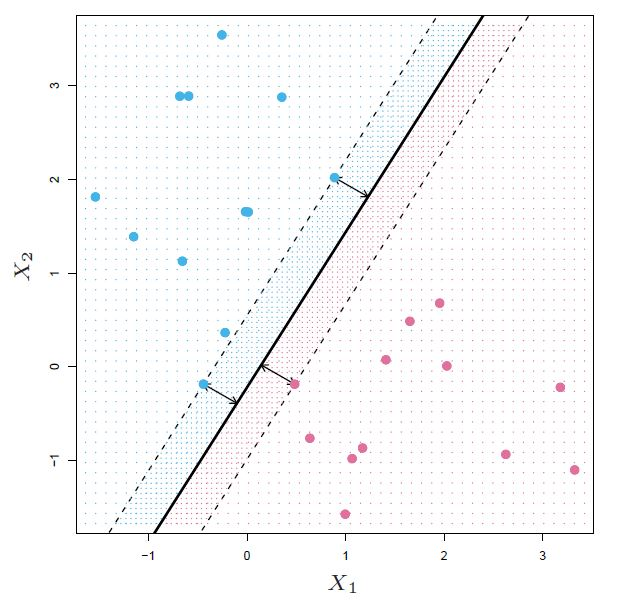
\includegraphics[width=0.7\textwidth]{PE4/svm.JPG}
\caption{Maximal margin hyperplane separating two classes of data points with the margin borders visualized by dotted lines}
\label{fig:mmh}
\end{figure}


\subsubsection{Support vector classifier}

....


An introduction to statistical learning

\subsection{Logistic regression}

Logistic regression is a algorithm for binary classification. The goal is to create a classifier which predicts the probability for a given data point $X$ to belong to a certain class $c$. This probability	 of a class $c$ under the condition of $X$ can be written as
\begin{equation} \label{eq:4}
p(c|X)
\end{equation}
The create model $h(X)=p(c=1|X)$  for a binary classification is the probability of a data point $X$ being of the class 1.
\\
Logistic regression is based on a (multiple) linear regression. Linear regression models a linear function which estimates a function of which data points are known for that the function holds as seen in equation \ref{eq:5}. 
\begin{equation} \label{eq:5}
y=\beta_0 + \beta_1 x_1 + \beta_2 x_2 + ... + + \beta_n x_n
\end{equation}

 The function parameters $\beta_1$ to  $\beta_n$ are estimated based on the given data points.  
To achieve an output with the domain of [0,1] for the hypotesis $h$ the logistic function is utilized:

\begin{equation} \label{eq:6}
f(x)=\frac{1}{1+e^-x}=\frac{e^x}{1+e^x}
\end{equation}



% https://www.jstor.org/stable/pdf/2983890.pdf?refreqid=excelsior:3ac2d6a000fa78f731ab46b8659528c0
D. R. Cox, The Regression Analysis of Binary Sequences 1958
\subsection{Decision tree}
% https://wiki.eecs.yorku.ca/course_archive/2014-15/F/4412/_media/ensemble_data_mining.pdf 54 (somewhere)
\subsection{Random forest}
% https://wiki.eecs.yorku.ca/course_archive/2014-15/F/4412/_media/ensemble_data_mining.pdf 54 (72)
\subsection{Gradient-boosted trees}
% https://wiki.eecs.yorku.ca/course_archive/2014-15/F/4412/_media/ensemble_data_mining.pdf 54 (somewhere)
\subsection{Naive Bayes}
% http://researchweb.watson.ibm.com/people/r/rish/papers/RC22230.pdf (IBM ressource)
info PDF in quellen